% `template.tex', a bare-bones example employing the AIAA class.
%
% For a more advanced example that makes use of several third-party
% LaTeX packages, see `advanced_example.tex', but please read the
% Known Problems section of the users manual first.
%
% Typical processing for PostScript (PS) output:
%
%  latex template
%  latex template   (repeat as needed to resolve references)
%
%  xdvi template    (onscreen draft display)
%  dvips template   (postscript)
%  gv template.ps   (onscreen display)
%  lpr template.ps  (hardcopy)
%
% With the above, only Encapsulated PostScript (EPS) images can be used.
%
% Typical processing for Portable Document Format (PDF) output:
%
%  pdflatex template
%  pdflatex template      (repeat as needed to resolve references)
%
%  acroread template.pdf  (onscreen display)
%
% If you have EPS figures, you will need to use the epstopdf script
% to convert them to PDF because PDF is a limmited subset of EPS.
% pdflatex accepts a variety of other image formats such as JPG, TIF,
% PNG, and so forth -- check the documentation for your version.
%
% If you do *not* specify suffixes when using the graphicx package's
% \includegraphics command, latex and pdflatex will automatically select
% the appropriate figure format from those available.  This allows you
% to produce PS and PDF output from the same LaTeX source file.
%
% To generate a large format (e.g., 11"x17") PostScript copy for editing
% purposes, use
%
%  dvips -x 1467 -O -0.65in,0.85in -t tabloid template
%
% For further details and support, read the Users Manual, aiaa.pdf.


% Try to reduce the number of latex support calls from people who
% don't read the included documentation.
%
\typeout{}\typeout{If latex fails to find aiaa-tc, read the README file!}
%


\documentclass[]{aiaa-tc}% insert '[draft]' option to show overfull boxes

 \title{Team 14 Project Technical Report for the 2017 IREC}

 \author{
  TEAM DUSTER%
  \\
  {\normalsize\itshape
   Swiss Federale Institute of Technology, Lausanne;
   Swiss Federale Institute of Techology, Zurich;School of Business and Engineering Vaud}
 }

 % Data used by 'handcarry' option if invoked
 \AIAApapernumber{YEAR-NUMBER}
 \AIAAconference{Conference Name, Date, and Location}
 \AIAAcopyright{\AIAAcopyrightD{YEAR}}

 % Define commands to assure consistent treatment throughout document
 \newcommand{\eqnref}[1]{(\ref{#1})}
 \newcommand{\class}[1]{\texttt{#1}}
 \newcommand{\package}[1]{\texttt{#1}}
 \newcommand{\file}[1]{\texttt{#1}}
 \newcommand{\BibTeX}{\textsc{Bib}\TeX}

\begin{document}

\maketitle

\begin{abstract}


The Project Technical Report shall contain an Abstract. At a minimum, the abstract shall identify the launch vehicle's mission/category in which the team is competing, identify any unique/defining design characteristics of launch vehicle, define the payload's mission (if applicable), and provide whatever additional information may be necessary to convey any other high-level project or program goals and objectives.


\end{abstract}

\section*{Nomenclature}

\begin{tabbing}
  XXX \= \kill% this line sets tab stop
  $J$ \> Jacobian Matrix \\
  $f$ \> Residual value vector \\
  $x$ \> Variable value vector \\
  $F$ \> Force, N \\
  $m$ \> Mass, kg \\
  $\Delta x$ \> Variable displacement vector \\
  $\alpha$ \> Acceleration, m/s\textsuperscript{2} \\[5pt]
  \textit{Subscript}\\
  $i$ \> Variable number \\
 \end{tabbing}

\section{INTRODUCTION}


The Project Technical Report shall contain an Introduction. This section provides an overview of the academic program, stakeholders, team structure, and team management strategies. The introduction may repeat some of the content included in the abstract, because the abstract is intended to act as a standalone synopsis if necessary.


\section{MISSION CONCEPT OF OPERATIONS OVERVIEW}

The Project Technical Report shall contain a Mission Concept of Operations (CONOPS) Overview. This section shall identify the mission phases, including a figure, and describe the nominal operation of all subsystems during each phase (eg a description of what is supposed to be occurring in each phase, and what subsystem[s] are responsible for accomplishing this). Furthermore, this section shall define what mission events signify a phase transition has occurred (eg "Ignition" may begin when a FIRE signal is sent to the igniter, and conclude when the propulsion system comes up to chamber pressure. Similarly, "Liftoff" may begin at vehicle first motion, and conclude when the vehicle is free of the launch rail). Phases and phase transitions are expected to vary from system to system based on specific design implementations and mission goals and objectives. No matter how a team defines these mission phases and phase transitions, they will be used to help organize failure modes identified in a Risk Assessment Appendix – described in Section 2.7.2.9 of this document.


\section{SYSTEM ARCHITECTURE OVERVIEW}

\subsection{Propulsion Subsystems}
\subsection{Aero-structure Subsystems}


\paragraph{Lower body}



\begin{figure}[h!]% order of placement preference: here, top, bottom
\centering
 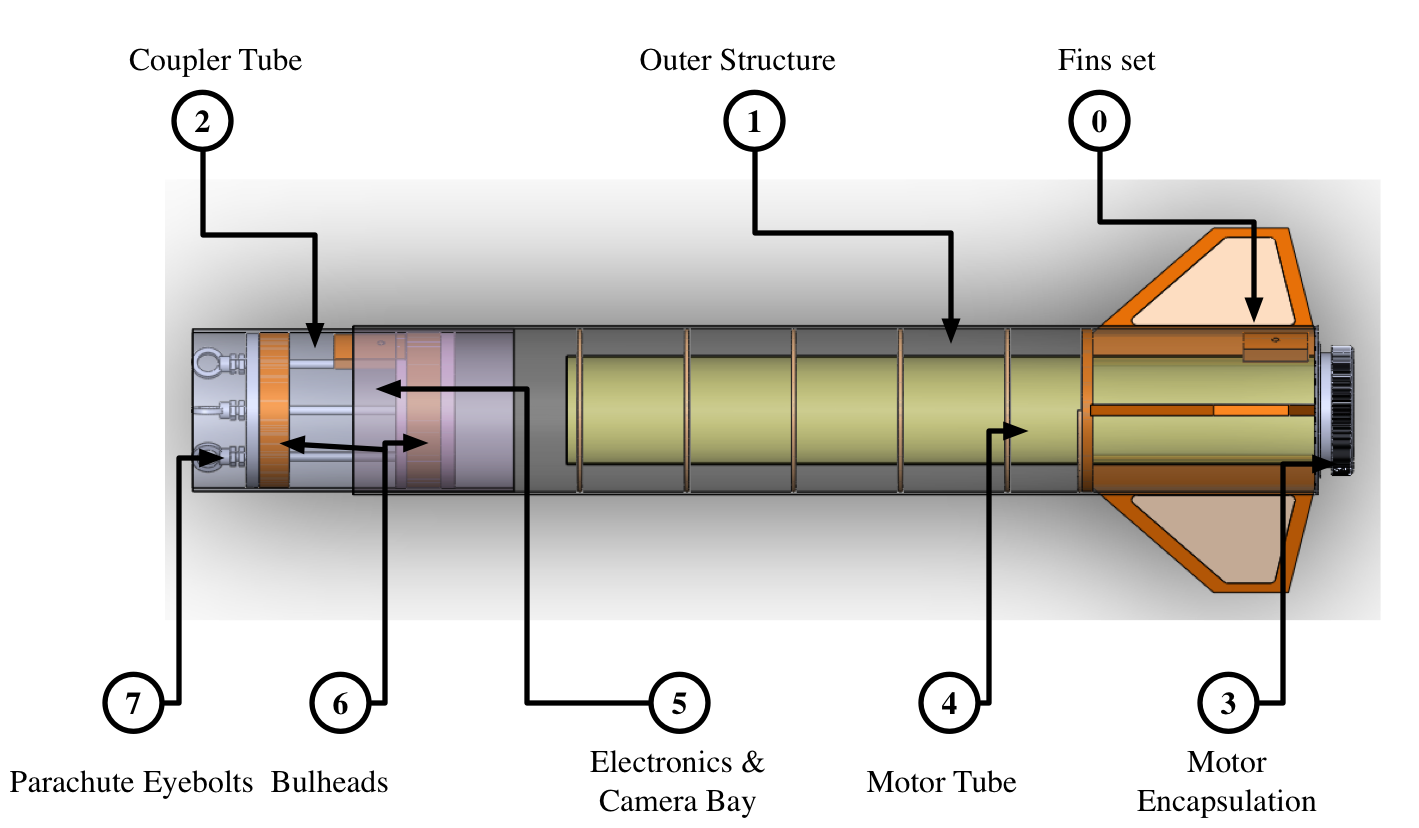
\includegraphics[width=0.8\textwidth]{images/PartsOfRocket}
 \caption{Lower body Main Components}
 \label{f:lower_body}
\end{figure}



\begin{enumerate}
\item Fins Set

Description:

\item Outer Structure

Description: 

Phenolic tube (temperature resistant) bought
\item Coupler tube

Description

\item Motor encapsulation

Description

\item Motor Tube

Description

\item Electronics and Camera Bay

Description:

\item Bulkheads 

- 250  3 layers of Carbon fibre on each side. 15 mm thick

\item Parachute Eyebolts



\end{enumerate}
Coupler Tube


Put the carbon fibre (two layers) without vacuum. 
Bulkhead inside the coupler tube.  3 x M8 rods and one in the centre. 


Holes for airventing


2 x M6 holes with a wood nut to mount the 2 x launch rails (take picture from Oliver) that are on the same part of rocket (on the lower body)



Apply epoxy on the inside, apply on the bulkhead and put them in. 



What to improve: 
- too many airventing holes, maybe we can make them smaller. holes are M5 x 6 => M3 x 6
- the bulkheads


\subsubsection{Upper body}

\subsubsection{Nosecose}

\subsection{Recovery Subsystems}

\subsection{Payload Subsystems}







\section{CONCLUSIONS AND LESSONS LEARNED}







\section{Model}

We should probably include some math.
Here we begin with Eq.~(\ref{e:function}) that demonstrates some math
typesetting.
\begin{equation}
 \label{e:function}
 \int_{0}^{r_{2}} F(r,\varphi) \, dr \, d\varphi =
    \left[ \sigma r_{2}/(2\mu_{0}) \right] \cdot
    \int_{0}^{\infty} \exp(-\rho|z_{j}-z_{i}|) \, \lambda^{-1} 
\end{equation}
Eq.~(\ref{e:function}) is grand.
Some say it is due to Rebek.\cite{rebek:82bk}

\section{Results}

In this section we will introduce some figures and tables.
It can be seen in figure~\ref{f:magnetic_field} that magnetization is a
function of applied field.

Sometimes writing meaningless text can be quiet easy, but other times
one is hard pressed to keep the words flowing.\footnote{And sometimes
things get carried away in endless detail.}
Meanwhile back in the other world, table~\ref{t:scheme_comparison} shows
a nifty comparison.
\begin{table}% no placement specified: defaults to here, top, bottom, page
 \begin{center}
  \caption{Variable and Fixed Coefficient Runge-Kutta Schemes as a
           Function of Reynolds Number}
  \label{t:scheme_comparison}
  \begin{tabular}{rrr}
       Re & Vary & Fixed \\\hline
        1 &  868 & 4,271 \\
       10 &  422 & 2,736 \\
       25 &  252 & 1,374 \\
       50 &  151 &   736 \\
      100 &  110 &   387 \\
      500 &   85 &   136 \\
    1,000 &   77 &   117 \\
    5,000 &   81 &    98 \\
   10,000 &   82 &    99
  \end{tabular}
 \end{center}
\end{table}


\clearpage
\section*{Appendix}



An appendix, if needed, should appear before the acknowledgments.
Use the 'starred' version of the \verb|\section| commands to avoid
section numbering.
\clearpage

\subsection*{Appendix 1 - System Weights, Measures and Performance Data}


\clearpage
\subsection*{Appendix 2 - Test Report}


\subsubsection{Recovery System Testing}

 In addition to descriptions of testing performed and the results thereof, teams shall include in this appendix a figure and supporting text describing the dual redundancy of recovery system electronics.

\clearpage
\subsection*{Appendix 3 - Hazard Analysis Appendix}


The third Project Technical Report appendix shall contain a Hazard Analysis. This appendix shall address as applicable, hazardous material handling, transportation and storage procedures of propellants, and any other aspects of the design which pose potential hazards to operating personnel. A mitigation approach – by process and/or design – shall be defined for each hazard identified.

\clearpage
\subsection*{Appendix 4 - Risk Assessment Appendix}

The fourth Project Technical Report appendix shall contain a Risk Assessment. This appendix shall summarize risk and reliability concepts associated with the project. All identified failure modes which pose a risk to mission success shall be recorded in a matrix, organized according to the mission phases identified by the CONOPS. A mitigation approach – by process and/or design – shall be defined for each risk identified. An example of such a matrix is available on the ESRA website at (http://www.soundingrocket.org/sa-cup-documents--forms.html).

\clearpage
\subsection*{Appendix 5 - Assembly, Preflight and Launch Checklists}

The fifth Project Technical Report appendix shall contain Assembly, Preflight, and Launch Checklists. This appendix shall include detailed checklist procedures for final assembly, arming, and launch operations. Furthermore, these checklists shall include alternate process flows for dis-arming/safe-ing the system based on identified failure modes. These off-nominal checklist procedures shall not conflict with the IREC Range Standard Operating Procedures (http://www.soundingrocket.org/sa-cup-documents--forms.html).
Competition officials will verify teams are following their checklists during all operations – including assembly, preflight, and launch operations. Therefore, teams shall maintain a complete, hardcopy set of these checklist procedures with their flight hardware during all range activities.


\clearpage
\subsection*{Appendix 6 - Engineering Drawings}

The sixth Project Technical Report appendix shall contain Engineering Drawings. This appendix shall include any revision controlled technical drawings necessary to define significant subsystems or components – especially SRAD subsystems or components.

\section*{Acknowledgments}

A place to recognize others.

\begin{thebibliography}{9}% maximum number of references (for label width)
 \bibitem{rebek:82bk}
 Rebek, A., {\it Fickle Rocks}, Fink Publishing, Chesapeake, 1982.
\end{thebibliography}

\end{document}

% - Release $Name:  $ -
